\documentclass[tikz,border=15pt]{standalone}
\usepackage{tikz}
\usepackage{amsmath}
\usepackage{amssymb}
\usetikzlibrary{positioning, arrows.meta, calc, backgrounds, fit, shapes.geometric}

\colorlet{color_intent}{blue!60!black}
\colorlet{color_slot}{green!50!black}
\colorlet{color_shared}{black!70}

\begin{document}

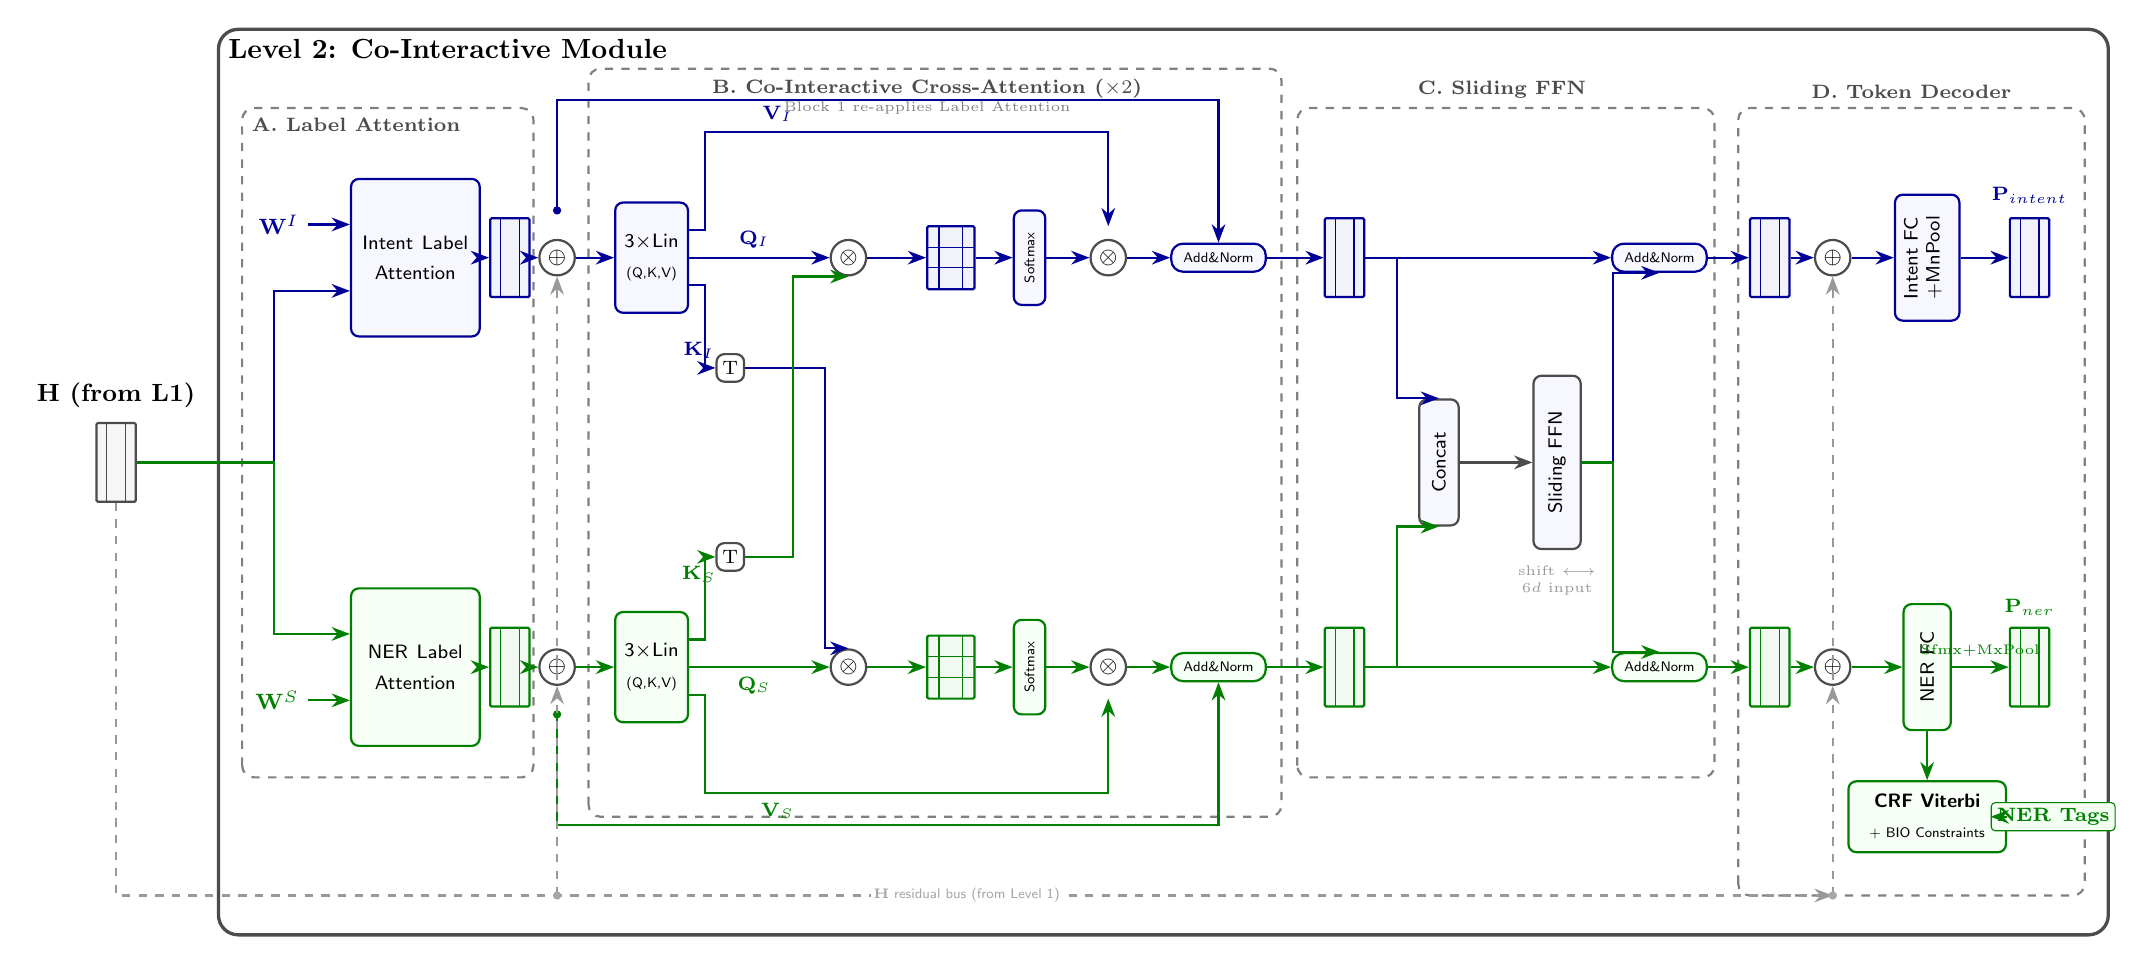
\begin{tikzpicture}[
    >=Stealth, font=\small\sffamily,
    mainbox/.style={draw=black!70, rounded corners=2.5mm, line width=1.2pt},
    subbox/.style={draw=black!50, dashed, rounded corners=1.5mm, line width=0.8pt},
    block/.style={draw=black!70, fill=white, rounded corners=1mm, thick, align=center},
    intent_block/.style={block, draw=blue!60!black, fill=blue!3},
    slot_block/.style={block, draw=green!50!black, fill=green!3},
    op/.style={circle, draw=black!70, fill=white, inner sep=0.5pt, minimum size=0.45cm, thick, font=\footnotesize},
    arrow/.style={->, thick, draw=black!70},
    arrow_intent/.style={->, thick, draw=blue!60!black},
    arrow_slot/.style={->, thick, draw=green!50!black},
    link_dashed_gray/.style={->, line width=1.0pt, dashed, draw=gray!80},
    matrix_vert/.style={
        draw=#1, thick, fill=#1!5, minimum width=0.5cm, minimum height=1.0cm, rounded corners=0.5pt,
        path picture={
            \draw[#1, thin] (-0.12,-0.5) -- (-0.12,0.5);
            \draw[#1, thin] (0.12,-0.5) -- (0.12,0.5);
        }
    },
    matrix_grid/.style={
        draw=#1, thick, fill=#1!5, minimum width=0.6cm, minimum height=0.8cm, rounded corners=0.5pt,
        path picture={
            \draw[#1, thin] (-0.15,-0.4) -- (-0.15,0.4);
            \draw[#1, thin] (0.15,-0.4) -- (0.15,0.4);
            \draw[#1, thin] (-0.3,-0.13) -- (0.3,-0.13);
            \draw[#1, thin] (-0.3,0.13) -- (0.3,0.13);
        }
    }
]

%% ============================================================
%% TIER 2: CO-INTERACTIVE FEATURE MINING
%% ============================================================
\draw[mainbox] (1.5, -1.0) rectangle (25.5, 10.5);
\node[anchor=north west, font=\bfseries] at (1.5, 10.5) {Level 2: Co-Interactive Module};

%% --- Input H (from Tier 1) ---
\node[matrix_vert=color_shared] (H_mat) at (0.2, 5.0) {};
\node[above=0.05cm of H_mat, font=\bfseries\small] {$\mathbf{H}$ (from L1)};


%% --- A. LABEL ATTENTION ---
\draw[subbox] (1.8, 1.0) rectangle (5.5, 9.5);
\node[anchor=north west, font=\bfseries\scriptsize, text=black!70] at (1.8, 9.5) {A. Label Attention};

\node[intent_block, minimum height=2.0cm, text width=1.4cm] (attn_I) at (4.0, 7.6) {\scriptsize Intent Label\\Attention};
\node[slot_block, minimum height=2.0cm, text width=1.4cm] (attn_S) at (4.0, 2.4) {\scriptsize NER Label\\Attention};

\node[font=\bfseries\footnotesize, text=color_intent, anchor=east] (WI) at ([xshift=-15pt, yshift=12pt]attn_I.west) {$\mathbf{W}^I$};
\node[font=\bfseries\footnotesize, text=color_slot, anchor=east] (WS) at ([xshift=-15pt, yshift=-12pt]attn_S.west) {$\mathbf{W}^S$};

\draw[arrow_intent] (WI.east) -- ([yshift=12pt]attn_I.west);
\draw[arrow_slot] (WS.east) -- ([yshift=-12pt]attn_S.west);

\draw[arrow_intent] (H_mat.east) -- (2.2, 5.0) |- ([yshift=-12pt]attn_I.west);
\draw[arrow_slot] (H_mat.east) -- (2.2, 5.0) |- ([yshift=12pt]attn_S.west);

\node[matrix_vert=color_intent] (mat_I1) at (5.2, 7.6) {};
\node[matrix_vert=color_slot] (mat_S1) at (5.2, 2.4) {};
\draw[arrow_intent] (attn_I.east) -- (mat_I1.west);
\draw[arrow_slot] (attn_S.east) -- (mat_S1.west);

%% --- +H RESIDUAL FROM TIER 1 ---
%% Code: block(H_I + H, H_N + H, mask)
\node[op] (plus_blk_I) at (5.8, 7.6) {$\oplus$};
\node[op] (plus_blk_S) at (5.8, 2.4) {$\oplus$};
\draw[arrow_intent] (mat_I1.east) -- (plus_blk_I.west);
\draw[arrow_slot] (mat_S1.east) -- (plus_blk_S.west);


%% --- B. CO-INTERACTIVE CROSS-ATTENTION (CORRECTED) ---
\draw[subbox] (6.2, 0.5) rectangle (15.0, 10.0);
\node[anchor=north, font=\bfseries\scriptsize, text=black!70] at (10.5, 10.0) {B. Co-Interactive Cross-Attention ($\times 2$)};
\node[font=\tiny, text=black!50, align=center] at (10.5, 9.5) {Block 1 re-applies Label Attention};

\node[intent_block, minimum height=1.4cm, minimum width=0.8cm] (lin_I) at (7.0, 7.6) {\scriptsize 3$\times$Lin\\\tiny(Q,K,V)};
\node[slot_block, minimum height=1.4cm, minimum width=0.8cm] (lin_S) at (7.0, 2.4) {\scriptsize 3$\times$Lin\\\tiny(Q,K,V)};
\draw[arrow_intent] (plus_blk_I.east) -- (lin_I.west);
\draw[arrow_slot] (plus_blk_S.east) -- (lin_S.west);

\node[op] (mul1_I) at (9.5, 7.6) {$\otimes$};
\node[op] (mul1_S) at (9.5, 2.4) {$\otimes$};

\node[block, minimum size=0.35cm, inner sep=1pt, font=\scriptsize] (T_I) at (8.0, 6.2) {T};
\node[block, minimum size=0.35cm, inner sep=1pt, font=\scriptsize] (T_S) at (8.0, 3.8) {T};

% === INTENT STREAM ===
\draw[arrow_intent] ([yshift=10pt]lin_I.east) -- ++(0.2,0) |- (12.8, 9.2) -- (12.8, 8.0);
\node[above, font=\scriptsize, text=color_intent] at (8.6, 9.2) {$\mathbf{V}_I$};
\draw[arrow_intent] (lin_I.east) -- (mul1_I.west);
\node[above, font=\scriptsize, text=color_intent] at (8.3, 7.6) {$\mathbf{Q}_I$};
\draw[arrow_intent] ([yshift=-10pt]lin_I.east) -- ++(0.2,0) |- (T_I.west);
\node[above, font=\scriptsize, text=color_intent] at (7.6, 6.2) {$\mathbf{K}_I$};
\draw[arrow_intent] (T_I.east) -- (9.2, 6.2) |- (mul1_S.north);

% === SLOT STREAM ===
\draw[arrow_slot] ([yshift=-10pt]lin_S.east) -- ++(0.2,0) |- (12.8, 0.8) -- (12.8, 2.0);
\node[below, font=\scriptsize, text=color_slot] at (8.6, 0.8) {$\mathbf{V}_S$};
\draw[arrow_slot] (lin_S.east) -- (mul1_S.west);
\node[below, font=\scriptsize, text=color_slot] at (8.3, 2.4) {$\mathbf{Q}_S$};
\draw[arrow_slot] ([yshift=10pt]lin_S.east) -- ++(0.2,0) |- (T_S.west);
\node[below, font=\scriptsize, text=color_slot] at (7.6, 3.8) {$\mathbf{K}_S$};
\draw[arrow_slot] (T_S.east) -- (8.8, 3.8) |- (mul1_I.south);

% Attention output
\node[matrix_grid=color_intent] (mat_I2) at (10.8, 7.6) {};
\node[intent_block, minimum height=1.2cm, minimum width=0.4cm] (soft_I) at (11.8, 7.6) {\rotatebox{90}{\tiny Softmax}};
\node[op] (mul2_I) at (12.8, 7.6) {$\otimes$};
\node[intent_block, rounded corners=1.5mm, minimum width=1.2cm] (addnorm1_I) at (14.2, 7.6) {\tiny Add\&Norm};

\node[matrix_grid=color_slot] (mat_S2) at (10.8, 2.4) {};
\node[slot_block, minimum height=1.2cm, minimum width=0.4cm] (soft_S) at (11.8, 2.4) {\rotatebox{90}{\tiny Softmax}};
\node[op] (mul2_S) at (12.8, 2.4) {$\otimes$};
\node[slot_block, rounded corners=1.5mm, minimum width=1.2cm] (addnorm1_S) at (14.2, 2.4) {\tiny Add\&Norm};

\draw[arrow_intent] (mul1_I.east) -- (mat_I2.west);
\draw[arrow_intent] (mat_I2.east) -- (soft_I.west);
\draw[arrow_intent] (soft_I.east) -- (mul2_I.west);
\draw[arrow_intent] (mul2_I.east) -- (addnorm1_I.west);
\draw[arrow_slot] (mul1_S.east) -- (mat_S2.west);
\draw[arrow_slot] (mat_S2.east) -- (soft_S.west);
\draw[arrow_slot] (soft_S.east) -- (mul2_S.west);
\draw[arrow_slot] (mul2_S.east) -- (addnorm1_S.west);

% Residual from ⊕ output (= label_attn + H) to Add&Norm
\fill[color_intent] (5.8, 8.2) circle (1.5pt);
\draw[arrow_intent] (5.8, 8.2) -- (5.8, 9.6) -| (addnorm1_I.north);
\fill[color_slot] (5.8, 1.8) circle (1.5pt);
\draw[arrow_slot] (5.8, 1.8) -- (5.8, 0.4) -| (addnorm1_S.south);


%% --- C. SLIDING WINDOW FFN ---
\draw[subbox] (15.2, 1.0) rectangle (20.5, 9.5);
\node[anchor=south, font=\bfseries\scriptsize, text=black!70] at (17.8, 9.5) {C. Sliding FFN};

\node[matrix_vert=color_intent] (mat_I3) at (15.8, 7.6) {};
\node[matrix_vert=color_slot] (mat_S3) at (15.8, 2.4) {};
\draw[arrow_intent] (addnorm1_I.east) -- (mat_I3.west);
\draw[arrow_slot] (addnorm1_S.east) -- (mat_S3.west);

\node[intent_block, draw=black!70, minimum height=1.6cm, minimum width=0.5cm] (concat) at (17.0, 5.0) {\rotatebox{90}{\scriptsize Concat}};
\node[intent_block, draw=black!70, minimum height=2.2cm, minimum width=0.6cm] (ffn) at (18.5, 5.0) {\rotatebox{90}{\scriptsize Sliding FFN}};
\node[font=\tiny, text=black!40, align=center] at (18.5, 3.5) {shift $\leftarrow\!\rightarrow$\\6$d$ input};

\node[intent_block, rounded corners=1.5mm, minimum width=1.2cm] (addnorm2_I) at (19.8, 7.6) {\tiny Add\&Norm};
\node[slot_block, rounded corners=1.5mm, minimum width=1.2cm] (addnorm2_S) at (19.8, 2.4) {\tiny Add\&Norm};

\draw[arrow_intent] (mat_I3.east) -- (addnorm2_I.west);
\draw[arrow_slot] (mat_S3.east) -- (addnorm2_S.west);
\draw[arrow_intent] (mat_I3.east) -- ++(0.4, 0) |- (concat.north);
\draw[arrow_slot] (mat_S3.east) -- ++(0.4, 0) |- (concat.south);
\draw[arrow] (concat.east) -- (ffn.west);
\draw[arrow_intent] (ffn.east) -- ++(0.4, 0) |- (addnorm2_I.south);
\draw[arrow_slot] (ffn.east) -- ++(0.4, 0) |- (addnorm2_S.north);


%% --- D. TOKEN DECODER (CORRECTED: +H skip connection before FC) ---
\draw[subbox] (20.8, -0.5) rectangle (25.2, 9.5);
\node[anchor=south, font=\bfseries\scriptsize, text=black!70] at (23.0, 9.5) {D. Token Decoder};

\node[matrix_vert=color_intent] (mat_out_I) at (21.2, 7.6) {};
\node[matrix_vert=color_slot] (mat_out_S) at (21.2, 2.4) {};
\draw[arrow_intent] (addnorm2_I.east) -- (mat_out_I.west);
\draw[arrow_slot] (addnorm2_S.east) -- (mat_out_S.west);

% +H before FC heads: code does intent_fc(H_I + H) and ner_fc(H_N + H)
\node[op] (plus_dec_I) at (22.0, 7.6) {$\oplus$};
\node[op] (plus_dec_S) at (22.0, 2.4) {$\oplus$};
\draw[arrow_intent] (mat_out_I.east) -- (plus_dec_I.west);
\draw[arrow_slot] (mat_out_S.east) -- (plus_dec_S.west);

\node[intent_block, minimum height=1.6cm, minimum width=0.6cm, align=center] (dec_I) at (23.2, 7.6) {
    \rotatebox{90}{\scriptsize Intent FC}
    \rotatebox{90}{\scriptsize +MnPool}
};
\draw[arrow_intent] (plus_dec_I.east) -- (dec_I.west);
\node[matrix_vert=color_intent] (P_I) at (24.5, 7.6) {};
\node[above=0.05cm of P_I, font=\bfseries\scriptsize, text=color_intent] {$\mathbf{P}_{intent}$};
\draw[arrow_intent] (dec_I.east) -- (P_I.west);

\node[slot_block, minimum height=1.6cm, minimum width=0.6cm, align=center] (dec_S) at (23.2, 2.4) {\rotatebox{90}{\scriptsize NER FC}};
\draw[arrow_slot] (plus_dec_S.east) -- (dec_S.west);

\node[matrix_vert=color_slot] (P_S) at (24.5, 2.4) {};
\node[above=0.02cm of P_S, font=\bfseries\scriptsize, text=color_slot] {$\mathbf{P}_{ner}$};
\draw[arrow_slot] (dec_S.east) -- (P_S.west) node[midway, above, font=\tiny, text=color_slot] {Sfmx+MxPool};

\node[slot_block, minimum height=0.9cm, minimum width=2.0cm, align=center] (crf_block) at (23.2, 0.5) {
    \scriptsize \textbf{CRF Viterbi}\\
    \tiny + BIO Constraints
};
\draw[arrow_slot] (dec_S.south) -- (crf_block.north);
\node[font=\scriptsize\bfseries, text=color_slot, fill=green!5, draw=green!50!black,
      rounded corners=0.5mm, inner sep=2pt] (ner_tags_out) at (24.8, 0.5) {NER Tags};
\draw[arrow_slot] (crf_block.east) -- (ner_tags_out.west);


%% --- H DISTRIBUTION BUS ---
\draw[link_dashed_gray, line width=0.8pt] (H_mat.south) -- (0.2, -0.5) -- (22.0, -0.5);
\node[font=\tiny\sffamily, text=gray!70, fill=white, inner sep=1pt] at (11.0, -0.5) {$\mathbf{H}$ residual bus (from Level 1)};

\draw[link_dashed_gray, line width=0.8pt] (5.8, -0.5) -- (plus_blk_I.south);
\draw[link_dashed_gray, line width=0.8pt] (5.8, -0.5) -- (plus_blk_S.south);
\fill[gray!70] (5.8, -0.5) circle (1.5pt);

\draw[link_dashed_gray, line width=0.8pt] (22.0, -0.5) -- (plus_dec_I.south);
\draw[link_dashed_gray, line width=0.8pt] (22.0, -0.5) -- (plus_dec_S.south);
\fill[gray!70] (22.0, -0.5) circle (1.5pt);

\end{tikzpicture}

\end{document}
